\DiaryEntry{Pythagorean Triples (cont'd)}{2023-04-11}{Number Theory}

The following Figure shows the distribution of primitive Pythagorean triples for values $x, y < 2500$.

\begin{figure}[H]
    \centering
    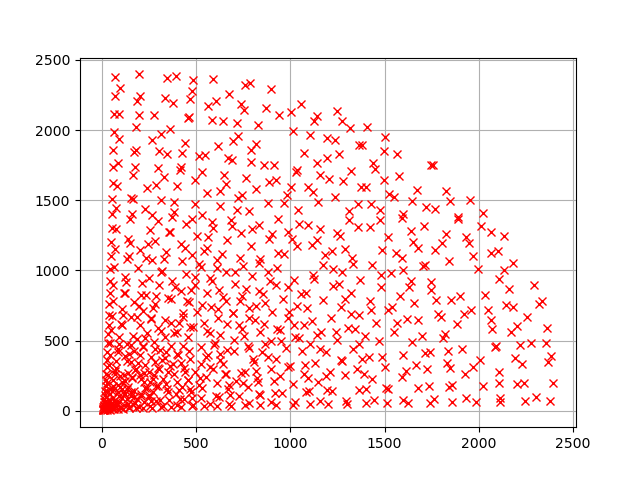
\includegraphics[scale=0.75]{images/2023-03-28-triples_2.png}
\end{figure}

In total, we have $395$ points out of a total $2500^2$ points; that corresponds to a density of $\approx 6.3 \cdot 10^{-5}$. In other words, it is highly unlikely to find a primitive Pythagorean triple by chance.

When we consider non-priitive Pythagorean triples as well, we obtain the following Figure.

\begin{figure}[H]
    \centering
    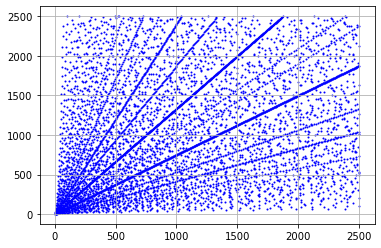
\includegraphics[scale=0.75]{images/2023-03-28-triples_3.png}
\end{figure}

From the lines in the Figure we can clearly see we can generate non-primitive Pythagorean triples $(kx, ky, kz)$ from a primitive triple $(x,y,z)$. This increates the number of points to $6004$; so we have a density of $\approx 9.6 \cdot 10^{-4}$.

Wikipedia holds some more interesting stuff. The expression

\bee
\frac{1}{2}(z-x)(z-y) = \frac{1}{2}(s^2+t^2 - 2st)(s^2+t^2-(s^2-t^2) = \frac{1}{2} (s-t)^2 2t^2 = t^2(s-t)^2
\eee

is a perfect square. Note that this is only a necessary condition not a sufficient one (i.e. a triple fulfilling the condition need not be a Pythagorean triple).

As an example, for the triple $(6, 12, 18)$, $\frac{1}{2}(z-x)(z-y) = \frac{1}{2} \cdot 12 \cdot 6 = 36$ is a perfect square, but it is not a (primitive) Pythagorean triple: $6^2 + 12^2 \neq 18^2$.

In addition, from above we see that $(z-x) = (s-t)^2$ is a perfect square as is $\frac{1}{2}(z-y) = t^2$. We can check this with the primitive Pythagorean triple $(8, 15, 17)$: $17 - 8 = 9 = 3^2$ and $\frac{1}{2} (17-15) = 1 = 1^2$. Again, this is not a sufficient condition as the example of $(8, 1, 9)$ shows.

In \ref{2023-03-28:entry}, Problem 9 we dealt with Pythagorean triples of the form $(x, y, x+1)$. Also interesting is the case $(x, x+1, z)$. These triples can be constructed by choosing consecutive Pell numbers for $s$ and $t$. The first few Pell numbers are $0, 1, 2, 5, 12, \cdots$ and choosing $s = 5, t=2$ we obtain the triple $(20, 21, 29)$.

\subsection{Pell Numbers}

Pell numbers $P_n$ \href{https://oeis.org/A000129}{sequence A000129 in the OEIS} are defined as follows,

\bee
P_n = 2 P_{n-1} + P_{n-2}, \quad P_0 = 0, P_1 = 1
\eee

which is of striking similarity as the Fibonacci numbers. A closed-form expression is given by

\bee
P_n = \frac{(1+\sqrt{2})^n - (1-\sqrt{2})^n}{2 \sqrt{2}}
\eee

The Pell numbers provide approximations for $\sqrt{2}$ as

\bee
\sqrt{2} \approx \frac{P_{n-1} + P_n}{P_n}
\eee

For example, 

\bee
\frac{P_7 + P_8}{P_8} = \frac{169 + 408}{408} \approx 1.414215686 = \sqrt{2} - 2.1239 \cdot 10^{-6}
\eee

which yields a very good approximation.

We can use the Pell numbers to construct Pythagorean triples of the form $(x, x+1, z)$ as shown in the example above for $s = 5, t=2$ which yields the triple $(20, 21, 29)$.

To prove this, we use induction: Assume that we construct a triple using $s_1 = P_{n-1}, t_1 = P_{n-2}$, we have

\begin{align*}
    x_1 &= 2P_{n-1} P_{n-2} \\
    y_1 &= P_{n-1}^2 - P_{n-2}^2
\end{align*}

and as induction start we have that

\be\label{2023-04-12:eq1}
y_1 - x_1 = P_{n-1}^2 - P_{n-2}^2 - 2 P_{n-1} P_{n-2} = 1
\ee

Now we use the next two Pell numbers $s_2 = P_{n}, t_2 = P_{n-1}$, to obtain the next triple as

\begin{align*}
    x_2 &= 2P_{n} P_{n-1} \\
    y_2 &= P_{n}^2 - P_{n-1}^2
\end{align*}

Now we calculate the difference, $y_2 - x_2$: We have

\bee
    y_2 - x_2 = P_{n}^2 - P_{n-1}^2 - 2P_{n} P_{n-1}
\eee

and want to show that this is equal to $1$. We somehow want to make use of the induction start \ref{2023-04-12:eq1}; to this end, we use the Pell number definition $P_n = 2 P_{n-1} + P_{n-2}$ and obtain

\begin{align*}
    y_2 - x_2 &= (2 P_{n-1} + P_{n-2})^2 - P_{n-1}^2 - 2(2 P_{n-1} + P_{n-2}) P_{n-1} \\
    &= 4 P_{n-1}^2 + 4 P_{n-1} P_{n-2} + P_{n-2}^2 - P_{n-1}^2 - 4 P_{n-1}^2 - 2 P_{n-1} P_{n-2} \\
    &= 2 P_{n-1} P_{n-2} + P_{n-2}^2 - P_{n-1}^2 \\
    &= - (P_{n-1}^2 - P_{n-2}^2 - 2 P_{n-1} P_{n-2} ) = -1
\end{align*}

This completes the proof; however, note that in the first triple $y_1 > x_1$, whereas $x_2 > y_2$; i.e. the position of the bigger value changes. In our example, we chose $s = 5, t=2$ from which we obtained the triple $(20, 21, 29)$. The next Pell number is then $2 \times 5 + 2 = 12$ and from $s = 12, t = 5$ we obtain the next triple $(120, 119, 169)$. 

\qed


%%% Local Variables:
%%% mode: latex
%%% TeX-master: "journal"
%%% End:
